\documentclass{article}
\usepackage{tikz}
\usetikzlibrary{arrows.meta}

\begin{document}

\begin{center}
    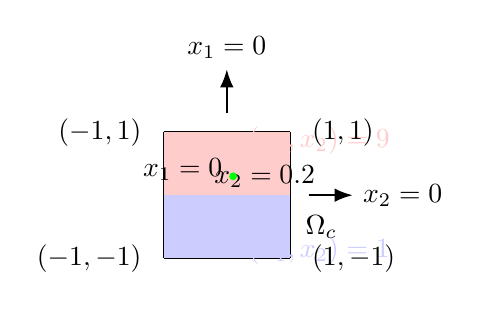
\begin{tikzpicture}[scale=0.8]
        % Domain boundaries
        \draw[thick] (-1,-1) -- (1,-1);
        \draw[thick] (-1,-1) -- (-1,1);
        \draw[thick] (1,-1) -- (1,1);
        \draw[thick] (-1,1) -- (1,1);

        % Region with c(x_1,x_2) = 9
        \fill[red!20] (-1,0) rectangle (1,1) node[pos=0.5,above right] {$c(x_1,x_2)=9$};

        % Region with c(x_1,x_2) = 1
        \fill[blue!20] (-1,-1) rectangle (1,0) node[pos=0.5,below right] {$c(x_1,x_2)=1$};

        % Labels
        \node at (-1.2,1) [left] {$( -1,1 )$};
        \node at (1.2,1) [right] {$( 1,1 )$};
        \node at (-1.2,-1) [left] {$( -1,-1 )$};
        \node at (1.2,-1) [right] {$( 1,-1 )$};
        \node at (-0.7,0.4) {$x_{1}=0$};
        \node at (0.6,0.3) {$x_{2}=0.2$};
        \node at (1.5,-0.5) {$\Omega_{c}$};
        \node at (0.1,0.3) [circle,fill=green,inner sep=1pt]{};

        % Axes labels
        \draw[-Latex, thick] (1.3,0) -- (2,0) node[right]{$x_{2}=0$};
        \draw[-Latex, thick] (0,1.3) -- (0,2) node[above]{$x_{1}=0$};
    \end{tikzpicture}
\end{center}

\end{document}